%umsetzung.tex
\chapter{Umsetzung}
\label{sec:Umsetzung}

\section{Datenaufbereitung}
Mit Hilfe des Python Modules \textit{psycopg2} werden die benötigten Daten aus der Datenbank nach Python importiert. 

\subsection{Tankstellendaten}
Der komplette Datensatz an Stammdaten zu den einzelnen Tankstellen wird als Instanzen der Klasse \textit{station} in einem \textit{dictionary} abgelegt, sodass jede Tankstelle über ihre \textit{id} abgerufen werden kann. Jedes einzelne Feld wird entweder übernommen oder - falls nicht verfügbar - mit einem Defaultwert gekennzeichnet. Der Großteil der benötigten Funktionalitäten wird über diese Klasse \textit{station} bereitgestellt.  

\subsection{Preisdaten}
Die für die Analyse benötigten Preisdaten einer Tankstelle werden in einer Matrix chronologisch gespeichert. Bis auf die Tanstellen-Id werden alle Felder übernommen. Der Zeitstempel wird in Zahlenwerte für das Datum und die Uhrzeit umgerechnet. Das Datum besteht in dem Abstand zum Datum der ersten Änderung in Tagen und die Uhrzeit in den an dem Tag vergangenen Sekunden. Aus dem Datum wird zusätzlich der Wochentag bestimmt und als Zahlenwert abgespeichert. Zu den jeweiligen aktuellen Preisen werden auch die Änderungsbeträge für jede Kraftstoffsorte ermittelt. Jede Form der Preisänderung wird bis auf einen Ausnahmefall so erhalten, wie sie ist. Die Struktur ist von Bedeutung, wenn es darum geht, inhaltlich zu bestimmen, welche Änderungen potentiell ein Auslöser sein könnten. Die Ausnahme ist, wenn Preise auf Null herabgesenkt werden. Diese Fälle würden extreme Differenzwerte erzeugen, welche in der Ermittelung der Schwellenwerte für die Regeln Fehler erzeugen könnten. Außerdem stellen sie inhaltlich keine wirkliche Preisänderung dar. In diesen Fällen wird für die entsprechende Kraftstoffsorte der bis dahin geltende Preis genommen. Würde durch diese Abwandlung ein Pricing entstehen, das keine Änderung beinhaltet, so wird der komplette Eintrag entfernt.

\section{Potentielle Konkurrenten ermitteln}
Wie in der Vorüberlegung angedeutet, soll hier zunächst eine grobe Auswahl der überhaupt als Konkurrenten in Frage kommenden anderen Tankstellen getroffen werden. Das Hauptkriterium hierfür soll der Abstand zur untersuchten Tankstelle sein, welcher über die Geokoordinaten bestimmt werden kann. Dafür wird der Einfachheit halber der direkte Abstand über die Erdkugel errechnet. Es ist allerdings nicht ausreichend einfach einen maximalen Abstandswert festzulegen und alle im Umkreis liegenden Tankstellen als potentielle Konkurrenten zu betrachten. Die Anzahl der umliegenden Tankstellen schwankt stark mit dem Besiedelungsgrad der unmittelbaren Umgebung und somit auch die maximalen Abstände von tatsächlichen Konkurrenten. So kann es in der Stadt durchaus vorkommen, dass der nächste Konkurent auf der anderen Straßenseite zu finden ist und sich noch 15 oder mehr weitere Tankstellen im Umkreis von wenigen Kilometern befinden, wohingegen es beispielsweise auf der Autobahn vorkommen kann, dass die nächste Tankstelle mehr als zehn Kilometer entfernt liegt.\\
In der aktuellen Version wird deshalb eine Mischung aus einer variablen Abstandsobergrenze und einer Mindest- und Maximalanzahl an potentiellen Konkurrenten verwendet. Solange im Umkreis der Abstandsgrenze nicht genügend Tankstellen gefunden wurden, wird die Obergrenze  immer wieder verdoppelt. Sollte die maximale Anzahl überschritten werden, so werden die am weitesten enfernt liegenden wieder entfernt. Die so ermittelten potentiellen Konkurrenten werden als Liste ihrer \textit{ids} nach dem Abstand geordnet in der derzeitig analysierten \textit{station}abgespeichert. Grund für die Wahl dieses Vorgehens, anstatt lediglich eine relativ hohe Mindestzahl festzulegen, ist, dass nicht unnötig viele Tankstellen ausgewählt werden sollen. Bei jeder Tankstelle besteht ein relativ hohes Risiko, Korrelationen zu finden, die über Interaktionen mit dritten Tankstellen hervorgerufen werden.

\section{Reaktionen erkennen}
Grundsätzlich wird hier durch die Preisänderungen der untersuchten Tankstelle und der potentiellen Konkurrenten durchiteriert und nach den im folgenden beschriebenen Kriterien werden Paarungen von potentiellen Reaktionen und deren Auslösern extrahiert. Dabei werden zunächst nur die Preissenkungen betrachtet. Außerdem kommen keine Parrungen in Frage, bei welchen zwischen Auslöser und Reaktion eine Erhöhung gelegen hat. Um den historischen Kontext auch später noch herleiten zu können, werden nicht die Daten der Paarungen an sich in einer List abgespeichert, sondern der jeweilige Index in den Matrizen, welcher die Daten enthält. Dabei wird je eine Liste für die potentiellen Konkurrenten erstellt, um schnell und einfach die Statistiken für die Regeln ableiten zu können. Zusätzlich werden alle potentiellen Auslöser einer Reaktion in Unterlisten gespeichert, welche chronologisch nach den Reaktionen sortiert werden, um später einfacher Auslöser untereinander vergleichen und ausschließen zu können.\\
Es geht an dieser Stelle noch nicht darum ausschließlich die genauen Auslöser der Preissenkungen einer Tankstelle zu finden. Dazu gibt es nicht ausreichend eindeutige Informationen. Es werden alle potentiellen Auslöser gesammelt um darüber anschließend mit statistischen Mitteln die wahrscheinlichsten Konkurrenten und die dazugehörigen Regeln ermitteln zu können. Dabei ist es unumgänglich  Änderungen als Auslöser zu interpretieren, die prinzipiell in Frage kämen, jedoch tatsächlich nicht wirksam wurden. Da die wirklichen Regeln mit ihren Preisschwellen noch nicht bekannt sind kann noch nicht gesagt werden, ob ein Auslöser überhaupt den Schwellenwert überschreitet. Unterschwellige Auslöser miteinzuschließen ist jedoch nicht ganz so kritisch, wie falsche Paarungen zu bilden, die höhere Differenzwerte als den Schwellenwert aufweisen. Das liegt daran, dass im weiteren Verlauf vom maximalen Differenzwert abwärts auf das Bestehen einer Regel geprüft wird. Wenn aufgrund von Fehlpaarungen systematisch höhere Differenzwerte als die Schwellenwerte entstehen würden, könnten dieser Wert bereits als Regel interpretiert werden, wodurch der wahre Regelwert nie betrachtet würde.\\
Falsche Paarungen könnten entstehen, wenn auf einem engen Zeitraum mehrere Senkungen vollzogen werden. Deswegen wird bei solchen Fällen eine extra Fallunterscheidung durchgeführt. Ausreißer kann es durch bewusste Regelverletzungen oder technische Ausfälle natürlich trotzdem geben. Diese sollten jedoch so vereinzelt auftreten, dass man sie als Ausreißer erkennen können sollte. Zunächst werden potentielle Reaktionen jedoch nach einer zeitlichen und einer semantischen Komponenten ausgewählt.

\subsection{Zeitliche Komponente}
Auslöser und Reaktion sollten zeitlich nahe beieinander liegen. Das heißt, es muss ein maximales Zeitfenster vor einer Preisänderung festgelegt werden, in welchem ein Pricing von einem potentiellen Konkurrenten als Auslöser in Frage kommt. In den letzten Monaten gab es häufig sechs bis acht Preisänderungen verteilt über ein Zeitintervall von weniger als 16 Stunden. Bei Reaktionen mit mehr als zwei Stunden Verzögerung wäre es also nicht unwahrscheinlich, dass die auslösende Tankstelle bereits eine erneute Senkung durchgeführt hat, bevor die Reaktion eintritt. Selbst bei einer Stunde würde bereits insgesamt mehr Zeit bei einem eigentlich ungewünschten Preisabstand verbracht werden als bei dem eigentlich angestrebten. Stark verzögerte Reaktionen sollten somit aus ökonomischer Sicht vermieden werden, um beim Kunden den Eindruck zu vermeiden, dass die Tankstelle verhältnismäßig teurer ist.\\
Trotzdem kann bei automatischen Pricing Tools eine Reaktionszeit eingestellt werden. Die in den Testdaten verwendeten Zeiten sind nicht größer als zehn Minuten. Andere Tankstellen könnten aber durchaus auch höhere Reaktionszeiten eingestellt haben. Tankstellen, die keine Pricing Tools benutzen, haben höchstwahrscheinlich generell eine höhere Reaktionszeit, weil erst manuell erkannt werden muss, dass eine Reaktion erforderlich ist. Zeitenfenster unter 20 Minuten zu verwenden, würde also mit ziemlicher Sicherheit einige Reaktionen nicht berücksichtigen. Um dem vorzubeugen wurde ein Zeitfenster von 45 Minuten gewählt. Ein zu großes Zeitfenster würde dazu führen, auch mehr korrelierende, aber nicht kausal verantwortliche, Preisänderungen in den Pool der potentiellen Auslöser aufzunehmen. Die 45 Minuten wurden gewählt um möglichst alle Auslöser und gleichzeitig möglichst wenige lediglich zeitlich korrelierende Preisänderungen zu erfassen.

\subsection{Semantische Komponente}
Inhaltlich sollte der Höhenbetrag der Preisänderung in allen geänderten Kraftstoffsorten bei der Reaktion kleiner oder gleich der Änderung des Auslösers sein. Das liegt daran, dass der Preisabstand vor einem Auslöser maximal dem Schwellenwert entspricht. Ein Auslöser kann den Schwellenwert also maximal um die Höhe seiner Änderung unterschreiten. Eine Reaktion, die den Schwellenwert wieder herstellt, darf also nicht höher ausfallen als der Auslöser selber. Hier wird auch deutlich, warum die verschiedenen Strukturen der Pricings beibehalten werden sollten und nicht etwa ein Datensatz für jede Kraftstoffsorte erstellt wurde. Entspricht nur eine Kraftstoffsorte einer Preisänderung nicht diesem notwendigen Kriterien, so kommt die ganze Änderung als regelkonforme Reaktion nicht mehr in Frage. Bei einzelner Betrachtung der Kraftstoffsorten wäre diese Verschärfung des Ausschlusskriterium nicht möglich gewesen.\\

\subsection{Fallunterscheidung}
Es gibt vier verschiedene Fälle, die durch die verschiedenartigen Strukturen im Pricing Verhalten aber noch verkompliziert werden. Generell soll es möglich sein, dass ein Auslöser mehrere Reaktionen hervorruft, und zwar maximal eine pro Kraftstoffsorte. Umgekehrt gilt das Gleiche, also dass mehrere Auslöser eine Reaktion hervorrufen. Das liegt daran, dass es denkbar wäre, dass sowohl bei manuellem Betrieb als auch in automatischen Systemen Preisänderung mit mehreren auf einmal geänderten Kraftstoffsorten in einzelne Preisänderungen aufspalten werden oder auch einzelne, kurz hintereinanderliegende Änderungen zu einer Einzelnen zusammengefügt werden. Ausgeschlossen ist jedoch, dass pro Auslöser-Reaktionen-Paarung ein Kraftstoff bei einer Partei mehrmals geändert wird. Bei manuellen Änderungen ist es zwar möglich, dass bei einer Anpassung Fehler unterlaufen und deswegen eine weitere hinzugefügt werden muss, doch sollten diese Fälle so vereinzelt sein, dass es das letztliche Ergebnis kaum beeinflussen sollte. Auslöser-Reaktionen-Paarungen können also maximal drei Änderungen pro Seite enthalten. Zudem können in einem Zeitfenster verschieden viele unabhängige Preisänderungen auf beiden Seiten stattfinden. Deshalb wird bei beiden zunächst unterschieden, ob es sich um eine einzelne Änderung handelt, oder ob in zeitlicher Nähe mehrere Preisänderungen auftreten. Das Ergebnis davon lässt sich dann in vier verschiedene Fälle aufteilen.

\begin{enumerate}
\item \textbf{ein Auslöser - eine Reaktion}\\
Diese ist die am häufigsten vorkommende und einfachste Variante. Hier muss nur die semantische Komponente überprüft werden. 
\item \textbf{ein Auslöser - mehrere Reaktionen}\\

In diesem Fall befinden sich nur eine einzelne potentiell auslösende Preisänderung, aber mehrere Preisänderungen der untersuchten Tankstelle in einem Zeitintervall. Die letztlich gewählte Reaktion sollte auf jeden Fall das semantische Kriterium erfüllen. Bei jeder Reaktion muss für die Überprüfung dieses Kriteriums jede vorherige Reaktion in diesem Zeitintervall auf die jeweilige Reaktion selber aufaddiert werden. Das hat folgenden Hintergrund. Falls eine der späteren Änderungen die tatsächliche Reaktion war, dann war sie trotz allen vorherigen, ohnehin schon durchgeführten Änderungen anscheinend immer noch erforderlich. Es wird hierbei davon ausgegangen, dass auch die automatischen Tools nach dem Abwarten der Reaktionszeit vor der Durchführung der eigenen Änderung noch einmal den zu ändernden Betrag überprüfen. Würden sie dies nicht tun, könnte das dazu führen, dass eine Tankstelle systematisch einen geringeren Preis als nötig fährt und somit Gewinne einbüßt, weil sie Senkungen durchführt die laut ihren Regeln nicht mehr notwendig sind. Deshalb werden die potentiellen Reaktionen, angefangen bei der Ersten, aufaddiert, bis das semantische Kriterium nicht mehr erfüllt wird. Die letzte Änderung, die das Kriterium noch erfüllt, wird als tatsächliche Reaktion eingestuft. Wenn durch diese Änderung alleine nicht alle Kraftstoffsorten, die beim Auslöser geändert wurden, abgedeckt sind, kann die davor gelegene hinzugenommen werden, sofern es dadurch nicht zu einer doppelten Senkung eines Kraftstoffes kommt. Da hier drei verschiedene Sorten untersucht werden, können also maximal noch zwei Änderungen dazugenommen werden.\\
Dieses verfahren ist nicht komplett fehlerfrei, da es nicht möglich ist, die früheren Reaktionen inhaltlich komplett auszuschließen. Die Früheren zu wählen würde aber bei einem Fehler einen höheren Schwellenwert unterstützen. Die späteren Reaktionen senken den Abstand auf eine niedrigere Differenz, weil die vorheringen Reaktionen den Preis bereits schon wieder abgesenkt hatten. Es ist somit sicherer, die Reaktionen zu nehmen, die bei gleichzeitigem Erfüllen des semantischen Kriteriums am spätesten sind, um nicht das Risiko einzugehen, falsche größere Schwellenwerte zu begünstigen.\\
\begin{figure}[H]
	\center
	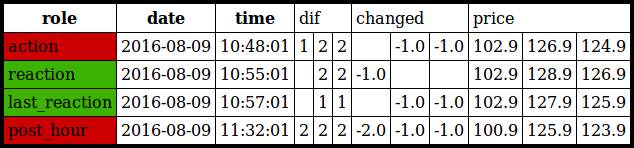
\includegraphics[width=0.6\textwidth]{Bilder/samr2.jpg}
	\caption{ein Auslöser - mehrere Reaktionen}
	\label{fig:SAMR}
\end{figure}
\autoref{fig:SAMR} beschreibt so einen Fall. Nur die spätere Reaktion kann die wahre Reaktion sein. Bei der Vorherigen ist die Anpassung bei Diesel höher als der Auslöser.

\item \textbf{mehrere Auslöser - eine Reaktion}\\
Der umgekehrte Fall, bei dem mehrere Änderungen eines Konkurrenten einer einzelnen Reaktion vorausgehen, lässt eine eindeutigere Entscheidung zu. In diesem Fall ist die letzte semantisch plausible Änderung des Konkurrenten der potentielle Auslöser. Angenommen, eine vorherige Änderung hätte die Reaktion ausgelöst, dann hätten alle noch folgenden Änderungen wiederum Reaktionen auslösen müssen. Es erfolgt jedoch offenbar nur eine Reaktion. Zudem ist diese Lösung wieder die sichere Variante. Bei den späteren Änderungen sind schon mehr Senkungen erfolgt, der Konkurrent hat also einen niedrigeren Preis. Die Reaktion stellt hier also einen verhältnismäßig niedrigen Schwellenwert wieder her. Sollte also der Fall eintreten, dass doch eine der früheren Änderungen der Auslöser war, und es wurde manuell eine weitere Senkung verhindert, so ist dies nicht nur ein von der Tankstelle gewollter Ausreißer, der auch als solcher bei der statistischen Auswertung keine Probleme bereiten sollte, sondern auch ein weniger kritischer Ausreißer, der die Wahl des Schwellenwertes nicht so stark beeinflusst.\\
Auch hier muss bei der Auswahl wieder berücksichtigt werden, dass eventuell mehrere Änderungen zusammen den Auslöser bilden. Die Auslöser werden deshalb von hinten durchiteriert. Handelt es sich bei dem aktuellen Auslöser um eine Änderung, bei der es bei den geänderten Kraftstoffsorten keinerlei Überschneidungen mit der Reaktion gibt, so kann diese Änderung übergangen werden. Das liegt daran, dass diese Änderung auch nicht eine erneute Änderung, wie oben beschrieben, hätte auslösen müssen. Sobald es eine solche Überschneidung gibt wird das semantische Kriterium überprüft. Wenn die Änderung mit dieser Überschneidung das semantische Kriterium noch nicht gänzlich erfüllt, können frühere hinzugenommen werden. Wieder dürfen dabei keine doppelten Änderungen einer Kraftstoffsorte entstehen, was bedeutet, dass wieder maximal zwei weiter Preisänderugnen als potentielle Auslöser dazugenommen werden können.
\begin{figure}[H]
	\center
	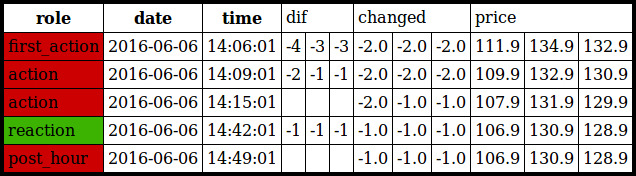
\includegraphics[width=0.6\textwidth]{Bilder/masr.jpg}
	\caption{mehrere Auslöser - eine Reaktion}
	\label{fig:MASR}
\end{figure}
In \autoref{fig:MASR} wird ein Beispiel für so einen Fall dargestellt. Von der Zeit her kommen alle Aktionen in Frage. Nach dem dritten Fall ist aber wahrscheinlich die letzte Aktion der wahre Auslöser. Hätten die Vorherigen Änderungen eine Reaktion erfordert, so hätte es für jede Nachfolgende ebenfalls eine Reaktion ausgelöst.

\item \textbf{mehrere Auslöser - mehrere Reaktion}\\
Die letzte Variante ist in der Umsetzung eine Kombination der vorherigen Fälle, was sich auch in der Begründung wiederspiegelt. Zunächst wird für die Kombination aller Auslöser untersucht, wieviele Reaktionen dadurch erklärt werden können. Dazu werden die Auslöser zu einem einzelnen künstlichen Auslöser zusammengefasst und dann die Reaktionen der Reihe nach addiert, solange das semantische Kriterium erfüllt bleibt. Sofern am Ende Reaktionen übrig bleiben, werden diese mit der selben Begründung wie im 2. Fall außer acht gelassen.\\

Die übrigen Reaktionen werden dann einzeln in rückwärtiger Reihenfolge untersucht, und gefundene Paarungen werden für die weitere Untersuchung gelöscht, sodass keine Doppelnennungen vorkommen können. Für die Betrachtung der jeweils letzten Reaktion, werden alle davorliegenden Auslöser gesammelt, und der 3. Fall wird angewendet. Das Entscheidungskriterium zugunsten des letzten möglichen Auslösers scheint hier außer Kraft gesetzt, denn spätestens ab der zweiten Iteration hatte es ja noch weitere spätere Reaktionen gegeben. Allerdings wurde für diese durch die rückwärtige Analyse bereits ein Auslöser gefunden oder es wurde bewiesen, dass es keinen semantisch möglichen Auslöser gibt, wodurch dieses Kriterium weiterhin gültig ist. Zudem gilt auch wieder, dass diese die sicherere Variante ist.\\

Wurden ein oder mehrere Auslöser für die aktuelle Reaktion gefunden, muss nur noch überprüft werden, ob weitere Reaktionen zwischen dem letzten der Auslöser und dieser aktuell letzten Reaktion liegen, die zusätzlich durch die gerade ausgewählten Auslöser erklärt werden können. Dabei kann es rein theoretisch wieder vorkommen, dass Auslöser, die zu einer späteren Reaktion passen, mit dieser gepaart und entfernt werden, obwohl sie eigentlich die Auslöser einer anderen, früheren Reaktion sind. Für diese Handhabung sprechen wieder die selben Gründe wie im 2. Fall. Wurde kein Auslöser gefunden, wird nur die gerade letzte Reaktion gelöscht.\\
\begin{figure}[H]
	\center
	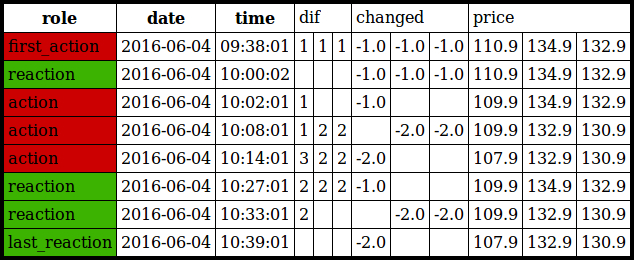
\includegraphics[width=0.6\textwidth]{Bilder/mamr3.jpg}
	\caption{mehrere Auslöser - mehrere Reaktion}
	\label{fig:MAMR}
\end{figure}
Das Reaktionsmuster in \autoref{fig:MAMR} ist ein relativ einfaches Beispiel so eines Falles, da die Reaktionen mittels der angepassten Werte eindeutig zu den Actionen gematched werden können. Davon kann jedoch nich immer ausgegangen werden.
\end{enumerate}

\section{Regeln spezifizieren}
Aus den gesammelten potentiellen Reaktionen sollen nun die in den Tools hinterlegten Regeln oder auch lediglich konsistente Verhaltensmuster abgeleitet werden. Dazu sollen die maximal zugelassene Preisabstände sowie die dazugehörigen Zeitintervalle erkannt werden. Letztlich muss dann über die ermittelten Regeln ermittelt werden, welche Tankstellen wirklich Konkurrenten sind. 

\subsection{Maximaler Preisabstand}
Die Verteilung der Preisdifferenz zweier Tankstellen ist das Hauptkriterium, auf welches sich die Klassifikation von Konkurrenz stützen wird. Wurde eine Regel und damit ein Schwellenwert für einen Konkurrenten hinterlegt, so sollte die Differenz nie lange über diesen Wert steigen. Es gibt zwei Möglichkeiten, wie eine Tankstelle auf die Änderung eines Konkurrenten entsprechend einer Regel reagieren kann. Entweder gar nicht, weil der Schwellenwert nicht überschritten wurde. Oder aber mit einer eigenen Preissenkung, wenn er überschritten wurde. Deshalb werden zwei verschiedene Differenzwerte unterschieden. Zum einen der Preisunterschied nach einer Änderung, auf die nicht reagiert werden musste. Der Maximalwert beschreibt hier den maximalen Abstand, auf den nicht reagiert werden musste. Gibt es eine Regel entspricht diese Differenz dem Schwellenwert. Zum anderen der Preisunterschied nachdem auf einen Konkurrenten reagiert werden musste. Für den Fall, dass es eine tatsächliche Reaktion und nicht nur eine Korrelation ist, sollte nach der reagierenden Preisänderung der Schwellenwert wieder hergestellt worden sein. Bei beiden Differenzen bestimmen die maximalen Werte den potentiellen Schwellenwert einer Regel. Um zu garantieren, dass genügend Daten für eine Analyse vorliegen, werden nur Konkurrenten analysiert, die mindestens ein Zehntel der Preisänderungen der untersuchten Tankstelle aufweisen.\\
Bei der Analyse dieser Werte werden die einzelnen Kraftstoffsorten zum ersten Mal komplett getrennt betrachtet. Werden bei einer Reaktion nicht alle Kraftstoffe angepasst, fällt diese Paarung für diese Sorte in die Kategorie, in der keine Reaktion notwendig war. Für jeden potentiellen Konkurrenten werden insgesammt je zwei Histogramme über die Preisunterschiede pro Kraftstoffsorte erstellt. Für das Histogramm über die Reaktionen müssen nur noch die Differenzwerte der gespeicherten Paarungen gebildet werden. Für das Histogramm über nicht erforderliche Reaktionen werden alle Preissenkungen des Konkurrenten ausgewählt, die nicht zu diesen Paarungen zählen. Jede dafür in Frage kommende Änderung wird noch einmal dahingehend überprüft, ob tatsächlich kein Pricing der untersuchten Tankstelle im anschließenden Zeitfenster zu finden ist. Durch das semantische Kriterium sind schließlich zeitlich korrelierende Anpassungen ausgeschlossen worden, weil sie keine Reaktionen darstellen. Es kann jedoch nicht mit Sicherheit gesagt werden, dass diese Änderung einen Preisabstand hergestellt hat, auf den nicht reagiert hätte werden müssen. Es könnte durchaus sein, dass eine Reaktion erforderlich gewesen wäre, hätte nicht ein anderer Konkurrent eine stärkere Reaktion bewirkt. Zudem müssen für die wirklich ignorierten Änderungen des Konkurrenten noch die zuletzt geltenden Preise der untersuchten Tankstelle ermittelt werden.\\
Die beiden Histogramme müssen dann für die Bestimmung des Maximalwertes zunächst zusammen betrachtet werden. Der dabei entstehende Maximalwert kann jedoch nicht sofort zum Schwellenwert gemacht werden. Es muss berücksichtigt werden, dass es durchaus noch sein kann, dass Tankstellen die Preise ohne Hilfe eines Tools anpassen oder zumindest die Anpassung selber noch manuell durchführen. Es kann also vorkommen, dass, obwohl eine Regel besteht, ab und zu dagegen verstoßen wird. Die Maximalwerte müssen also zunächst auf Ausreißer überprüft werden. Es wird also letztlich überprüft, ob die Häufigkeit, mit der ein entsprechender Wert auftritt, regelmäßig genug ist, um eine Vermutung von konkurrierendem Verhalten zu stützen. Diesbezüglich kann es durchaus vorkommen, dass zu einer Tankstelle eine Regel hinterlegt wurde, welcher nur sehr selten eine Reaktion erfordert. Ein Grund dafür könnte sein, dass der entsprechende Konkurrent selber in erster Linie auf die gerade untersuchte Tankstelle reagiert. Extremfälle dieser Art können nicht berücksichtigt werden, da ansonsten zu viele Ausreißer ebenfalls als Regel interpretiert werden würden.\\
Zusätzlich gilt es noch zu berücksichtigen, dass, sollte ein Wert zurückgewiesen werden, alle Differenzwerte,die diesen Schwellenwert gestützt hätten, zu Regelverstößen werden würden. Es gibt hierzu allerdings tankstellenübergreifend keine Erfahrungswerte, wie oft gegen Regeln verstoßen wird. Es ist durchaus möglich, dass sich dieser Faktor zwischen verschiedenen Unternehmen stark unterscheidet. Grundsätzlich sollte aber davon ausgegangen werden können, dass sich größententeils an Regeln gehalten wird, da diese Regeln im Allgemeinen einer ökonomischen Optimierung entstammen sollten, und Verstöße generell eine Gefahr bergen, Kunden zu verlieren.\\
Zuletzt ist es auch möglich für eine Tankstelle ihre Regeln auf bestimmte Zeit zu begrenzen, wodurch die Anzahl der zugehörigen Reaktionen auch deutlich geringer ausfallen kann. Diese drei Faktoren sprechen dafür, schon bei einer recht geringen Anzahl an unterstützenden Preismeldungen eine Regelmäßigkeit zu vermuten. Als Grenzwertfunktion wurde dafür diese Funktion gewählt:
\begin{center}
$ \frac{2}{\pi}*\arctan(2*\frac{x^2}{y})$\\
\end{center}
X stellt dabei die Häufigkeit dar, wie oft der entsprechende Differenzwert aufgetreten ist, und Y die Menge an Preismeldungen der Tankstelle im Allgemeinen. Als erste Richtlinie sollte der Grenzwert relativ zu der absoluten Menge der in diesem Zeitintervall liegenden Preisänderungen gewählt werden. Um die Häufigkeit des Wertes stärker zu gewichten, wird diese zunächst quadriert, bevor sie dann relativiert wird, damit bei moderat hohen Häufigkeiten eine unverhältnismäßig höhere absolute Anzahl an Preisänderugen nötig wäre, um diesen Wert zurückzuweisen. Angenommen, es würde einfach eine Prozenthürde von 10\% gewählt, so würde bei einer einzelnen entsprechenden Preisänderung aus zehn bereits ein Regel vermutet werden, wohingegen 9 aus 100 als Regel zurückgewiesen werden würden. Mit dem Arkustangens und den zusätzlichen Faktoren soll der errechnete Wert in einen Konfidenzwert zwischen 0 und 1 umgerechnet werden, der somit als Wahrscheinlichkeit interpretiert werden kann. Der Arkustangens garantiert dabei, dass die geringen Werte kaum verändert werden, wohingegen bei den hohen Werten der quadratische Faktor wieder etwas ausgeglichen wird. Die errechneten Konfidenzwerte lassen so trotz der verschieden großen Anzahlen an Preisänderungen zwischen den potentiellen Konkurrenten einen relativ guten Vergleich zwischen verschiedenen Regeln zu. Bei einem Maximalwert wird ab einer Häufigkeit, die einem Konfidenzwert größer als 0.5 entspricht, eine Regelmäßigkeit vermutet. Da es möglich ist, dass Tankstellen für einen Konkurrenten mehrere Regeln mit unterschiedlichen Schwellenwerten zu unterschiedlichen Zeiten erstellen, kann es durchaus vorkommen, dass neben dem maximalen Schwellenwert auch niedrigere Werte noch Regeln darstellen. Deshalb wird bei potentiellen Regeln zunächst überprüft, in welchem Zeitfenster sie gültig sind. Solange noch Zeitslots existieren, in denen noch keine Regel befolgt wird, werden die nächst niedrigeren Differenzwerte untersucht. 

\subsection{Zeitintervall}
Für jeden möglichen Maximalwert müssen nun die Zeitintervalle ermittelt werden, in denen dieser Wert auftritt. Sie definieren das Zeitfenster der Regel. In einem ersten Ansatz sollten die Regeln zunächst von den Zeitintervallen ausgehend erstellt werden, statt zunächst die Schwellenwerte zu errechnen. Die Daten sollten dafür rekursiv in immer kleinere Zeitintervalle aufgespalten werden. Anschließend sollte für jedes Intervall aus den darin liegenden Daten die Schwellenwerte, wie oben beschrieben, errechnet werden. Zuletzt sollten die Slots mit gleichen Abstandswerten zusammengefügt werden um wieder größere Intervalle zu bilden. Dies hat dazu geführt, dass bereits beim Versuch, die Daten nach einzelnen Wochentagen oder Stunden zu spalten, zu wenig Daten für die einzelnen Intervalle zur Verfügung standen, um halbwegs sichere Aussagen treffen zu können. Auch sind nicht so hochfrequente Konkurrenzmuster gänzlich unerkannt geblieben. In den zu Testzwecken zur Verfügung stehenden Regeln gibt es zwar nur wenige Einzelfälle, bei denen überhaupt eine zeitliche Unterscheidung von Schwellenwerten getroffen wurde. Es muss aber auch hier berücksichtigt werden, dass diese Testwerte nicht umbedingt repräsentativ für den ganzen Kraftstoffmarkt sind und andere Tankstellen durchaus feinere Unterscheidungen treffen könnten. Aus diesem Grund musste dieser Ansatz verworfen werden.\\
Stattdessen wird zunächst ein Tage- und Stundenübergreifend gültiger Schwellenwert vermutet. Deswegen werden die Differenzhistogramme wie oben beschrieben über den gesamten Zeitraum gebildet. Anschließend wird ermittelt, in welchen Zeitintervallen dieser Maximalwert auftritt. Hierbei wird nur einzeln entweder nach ganzen Tagen oder nach Stunden unterschieden. Es könnte sein, dass detailliertere Regeln für kleinere Stundeunintervalle an einzelnen Tagen existieren. Es ist aber relativ unwahrscheinlich, dass so eine feine Unterscheidung allzu häufig getroffen wird. Schließlich sollte es für jede weitere Aufsplittung eine ökonomische Rechfertigung geben. Es ist unwahrscheinlich, dass Kunden die Tankstellenpreise so genau verfolgen, dass sie die Preisabstände zu jeder Tages- und Uhrzeit kennen. Es müsste also ein gänzlich andere Art von Kundenaufkommen für diese speziellen Intervalle vermutet werden, die anderer Preisabstände rechtfertigen. Und selbst, wenn solche Unterschiede weit verbreitet wären, wäre eine detailliertere Analyse aufgrund der Dichte der Daten einfach kaum möglich.

\subsubsection{Potentielle Zeitintervalle ermitteln}
Dafür müssen zunächst alle möglichen Zeitslots für Tage und Stunden ermittelt werden. Dies sind die Zeiten, zu denen jeweils die untersuchte Tankstelle und der Konkurrent gleichzeitig geöffnet haben. Wie eben angesprochen werden nur die einzelenen Tage und tageübergreifend eine Stundenanzahl ermittelt. Es würden also auch keine unterschiedlichen Öffnungszeiten an Wochenenden berücksichtigt werden. Es gilt dann die längste Öffnungszeit der Woche. Die Öffnungszeiten der Tankstellen stehen in dem Datensatz von Tankerkönig nicht zur Verfügung. Allerdings reicht es auch, zu ermitteln, in welchen Zeitslots beide Tankstellen Preisänderungen durchführen, da diese Slots ohnehin auch nur die Zeitslots sind, bei denen Daten zur Verfügung stehen. Es ist außerdem besonders wichtig, dass jeder Zeitslot auch Daten hat, an denen er untersucht werden kann, da so lange weitere Schwellenwerte überprüft werden, bis alle Slots belegt sind. Auch hier müssen deswegen wieder Ausreißer berücksichtigt werden. Bei beiden Kategorien - Tagen und Stunden - werden die \textit{Öffnungszeit} für die in der Analyse betrachteten Tankstellen getrennt ermittelt und anschließend die der untersuchten Tankstelle mit dem jeweiligen Konkurrenten kombiniert.\\
Zur Bestimmung der geöffneten Tage wird der Mittelwert an Preisänderungen berechnet. Dabei fließen nur Tage in die Berechnung mit ein, an denen überhaupt Änderungen stattfinden. Ein Tag muss ein Zehntel dieses Mittelwertes überschreiten, um als gültiger Tagesslot zu gelten. Das ist notwendig, um einerseits Ausreißer auszuschließen und andererseits gewährleisten zu können, dass die Analyse des jeweiligen Maximalwertes für jeden Tag genügend zugrunde liegende Daten aufweist. Die Bestimmung der Stunden läuft bis dahin äquivalent ab. Allerdings müssen hier neben den positiven Ausreißern, also Preisänderungen zu Zeiten, in denen die Tankstelle eigentlich nicht geöffnet ist, aber aus irgendwelchen Gründen trotzdem Preise geändert werden auch negativ Ausreißer, also Zeiten in denen die Tankstelle geöffnet hat aber nur sehr wenige oder gar keine Preissenkungen vornimmt, berücksichtigt werden. Auch hier werden die Erhöhungen herausgenommen, da diese oftmals zu Randzeitpunkten wie zu Beginn oder am Ende einer Öffnungsperiode stattfinden und dabei öfters aus der tatsächlichen Öffnungszeit herausfallen. Für jede Stunde werden bei der Entscheidung zusätzlich jeweils die drei vorherigen und folgenden Stunden berücksichtigt. Für das vorangegangene und nachfolgende Intervall werden jeweils die Stunden gezählt, bei denen der Grenzwert von einem Zehntel vom Mittelwert überschritten wurde. Wird bei der betreffenden Stunde selber dieser Wert überschritten, so wird das Maximum dieser beiden Randintervalle gewählt und für die Entscheidung wird überprüft, ob mindestens zwei der drei Stunden ebenfalls diesen Wert überschreiten. Wird der Wert für die Stunde selber nicht erreicht, so wird das Minimum der Randintervalle dem gleichen Test unterzogen. Dieses Verfahren hat den Hintergrund, dass bei den Testtankstellen innerhalb der Öffnungszeiten Intervalle von zwei Stunden auftreten können, zu denen es kaum oder selten auch mal keine Änderungen gibt. Hier konnte auch repräsentativ getestet werden, da die Öffnungszeiten generell öffentlich zugänglich sind. Dieses Verfahren ermöglicht es diese Stunden trotzdem in die Analyse mit einzuschließen und gleichzeitig die Ränder nicht zu vergrößern. Zwar gibt es für diese auf diese Weise miteingeschlossenen Stunden keine Daten, was aber nicht problematisch ist, weil diese Fälle im weiteren Verlauf auch wieder berücksichtigt werden.

\subsubsection{Konkrete Zeitintervalle für Regeln definieren}
Wenn die möglichen Zeitslots feststehen, muss für die Schwellenwerte bezüglich eines Konkurrenten ein Gültigkeitsbereich definiert werden. Diese Slots ergeben sich durch die Verteilung derjenigen Reaktionen und ignorierten Preisänderungen, die exakt diesen gerade untersuchten Maximalwert generiert haben. Deshalb wird noch einmal ein Tages- sowie Stundenhistogramm für genau diejenigen Änderungen erstellt, die in diese Kategorie fallen. Es kann sein, dass dieser Schwellenwert nicht in jedem Slot vorkommt. Diejenigen Slots, bei denen nicht genügend Reaktionen oder ignorierten Preisänderungen mit Differenzen in dieser Höhe existieren, sind Kandidaten für eine weitere schwächere Regel.\\
Damit ein Zeitslot den aktuellen Schwellenwert zugewiesen bekommt, müssen ähnliche Probleme wie auch schon bei der Analyse der generell verfügbaren Slots, bedacht werden. Bei der Festlegung der Tage sind die Werte noch dicht genug, dass vom Ablauf her das gleiche Verfahren durchgeführt wird, mit dem einzigen Unterschied, dass diesmal nicht alle Preisänderungen in Frage kommen, sondern nur die dem aktuellen Schwellenwert zugehörigen. Wegen dieser Einschränkung der Datenmenge muss die Analyse bei den Uhrzeiten noch einmal abgewandelt werden. Das Pricingverhalten ist auch bei normalem, regelkonformem Verhalten hier bereits größeren Schwankungen unterlegen. Der Grenzwert, ab dem ein Slot belegt wird, ist deshalb abhängig von der Relation, der in diesem Slot liegenden Änderungen, welche die gerade getesteten Höhe aufweisen, zu der Gesammtheit aller in diesem Slot liegenden Preisänderungen. Der Anteil sollte 10\% nicht unterschreiten. Auch hier müssen wieder die Schwankungen berücksichtigt werden. Um nicht stark fluktuierende Regeln zu generieren, das heißt im Extremfall solche, die jeweils immer nur für einzelne Stunden gültig sind, wird die Mindestgültigkeitsdauer einer Regel auf 3 Stunden gesetzt. Daraus ergibt sich, dass sowohl einzelne Slots zusätzlich aufgenommen, als auch trotz hoher Werte zurückgewiesen werden können. Für die Umsetzung wird ein fünf Slots großer Kernel über die Liste der Uhrzeiten laufen gelassen wird, der die Belegung des einzelnen Slots im Zentrum danach auswählt, ob mehr oberschwellige oder mehr unterschwellige Werte in diesem Kernel liegen. Nach diesem Schritt sind für jeden Konkurrenten die möglichen Regeln eindeutig definiert.

\subsection{Klassifikation Konkurrenz}
Das Finden einer Regel bedeutet allerdings noch nicht die Existenz einer Konkurrenz. Bei der Entscheidung zugunsten einer Regel wurden schließlich nicht nur Reaktionen sondern auch die ignorierten Preisänderungen berücksichtigt. Der Konfidenzwert der Regel gibt nur an, dass, sollte überhaupt eine Regel zu dem jeweiligen Konkurrenten bestehen, dann sollte dieser Abstandswert mit der Sicherheit dieses Wertes eine Regel darstellen. Es kommt deshalb häufig vor, dass zwar hohe Sicherheiten bezüglich einer Regel bestehen, diese aber keine oder kaum Reaktionen erzeugt, weil der entsprechende potentielle Konkurrent eben kein wirklicher Konkurrent ist. Die hohe Sicherheit kommt dann dadurch zustande, dass der Abstandswert häufig zustande gekommen ist, ohne dass die untersuchte Tankstelle darauf reagieren wollte.\\
Um eine andere Tankstelle als Konkurrenten zu klassifizieren, muss also ein anderer Konfidenzwert berechnet werden. Der Einfachheit halber wurde hier der Anteil der Preissenkungen der untersuchten Tankstelle genommen, welcher durch die ermittelten Regeln gegenüber einem Konkurrenten hervorgerufen worden sein könnte. Das ist die Summe der Reaktionen jeder einzelnen Regel geteilt durch die Anzahl an Preissenkungen der untersuchten Tankstelle. Das hat den Hintergrund, dass ein tatsächlicher Konkurrent auch häufiger Reaktionen hervorrufen sollte, um als solcher gelten zu können. Wenn es trotzdem Fälle gibt, in denen Konkurrenten im System hinterlegt wurden, die kaum Reaktionen erzeugen, dann wäre es auch nicht besonders schädlich diese nicht als Konkurrenten zu klassifizieren, da die so falsch erklärten Preissenkungen sich auf einige wenige belaufen würden. Der Threshold wird dabei zunächst relativ niedrig auf drei Prozent gesetzt, um möglichst alle Konkurrenten zu erkennen. Die Erkennungsrate auf diese Weise hochzutreiben bringt natürlich eine hohe Wahrscheinlichkeit von $\alpha$ -Fehlern mit sich, also Fälle, in denen Konkurrenzen vermutet werden, wo eigentlich gar keine existieren. Diese Art von Fehlannahme hat auch noch weitere begünstigende Faktoren. Es ist in dieser Version noch nicht ausgeschlossen, dass für eine Reaktion verschiedene Auslöser von verschiedenen Tankstellen jeweils in deren Regeln mitgezählt werden. Die Summe der ermittelten Reaktionpaarungen über alle Konkurrenten hinweg kann also deutlich größer sein als die Anzahl der Reaktionen an sich. Die Auswirkungen dieser Faktoren werden in der folgenden Diskussion der Ergebnisse dargestellt.